\documentclass[
    iict, % Saisir le nom de l'institut rattaché
    il, % Saisir le nom de l'orientation
    %confidential, % Décommentez si le travail est confidentiel
]{heig-tb}

\usepackage[nooldvoltagedirection,european,americaninductors]{circuitikz}
\usepackage{lscape}
\signature{mbernasconi.svg} % Remplacer par votre propre signature vectorielle.

\makenomenclature
\makenoidxglossaries
\makeindex

\addbibresource{bibliography.bib}

\input{nomenclature}
\input{acronyms}
\input{glossary}
% Auteur du document (étudiant-e) en projet de Bachelor
\author{Nelson Jeanrenaud}

% Activer l'option pour l'accord du féminin dans le texte
\genre{male}

% Titre de votre travail de Bachelor
\title{Machine Learning pour prendre la décision d'un arrêt au stand en Formule 1}

% Le sous titre est optionnel
\subtitle{Rapport Intermédiaire Travail de Bachelor}

% Nom du professeur responsable
\teacher {Pena Carlos Andrés (HEIG-VD)}

% Mettre à jour avec la date de rendu du travail
\date{\today}

% Numéro de TB
\thesis{7212}



\surroundwithmdframed{minted}

%% Début du document
\begin{document}
\selectlanguage{french}
\maketitle
\frontmatter
\clearemptydoublepage

%% Requis par les dispositions générales des travaux de Bachelor
\preamble
\authentification

%% Résumé / Résumé publiable / Version abrégée
\begin{abstract}
    % Francais
L'objectif d'une course automobile est de parcourir un nombre de tours sur un circuit le plus
rapidement possible. De plus, dans de nombreuses catégories, les voitures peuvent s'arrêter au stand pour changer de pneus et/ ou se réapprovisionner en carburant.
La dégradation des pneus et le poids supplémentaire dû à la charge de carburant ont un impact majeur sur les temps au tour d'une voiture.
Décider quand et combien de fois rentrer dans les stands est donc crucial pour les écuries. À cela vienne s'ajouter les notions de neutralisation de la course pour cause d'incident.

Établir la stratégie optimale est un enjeu majeur pour les équipes de course. Il est donc nécessaire de développer un système d'analyse de données et de prédiction pour aider les écuries à prendre les meilleures décisions stratégiques pendant la course.
Ce système devra prendre en compte les données de la voiture, les performances des pneus et les conditions de la piste pour fournir des recommandations en temps réel aux équipes de course.

Dans ce travail, nous tentons de créer un tel système pour le championnat du monde de Formule 1.
Pour ce faire, nous entraînons des modèles de Machine Learning sur des données historiques de la dernière ère de la formule 1.

Un set de données a été établi à partir des données transmises par la Formule 1 pendant les courses.
Ces données ont été préparées de manière à former un ensemble complet et cohérent, permettant d'entraîner des modèles

Après l'expérimentation avec des réseaux de neurones et des réseaux de neurones récurrents,
nous avons réussi à développer des modèles capables de capturer les relations entre la stratégie de course et les données de la voiture.

Pour améliorer le système, nous pourrions inclure les facteurs météorologiques, développer une simulation de course pour améliorer la précision des prédictions
et tester l'apprentissage par renforcement pour développer des stratégies novatrices.
\end{abstract}

%% Sommaire et tables
\clearemptydoublepage
{
    \tableofcontents
    \let\cleardoublepage\clearpage
    \listoffigures
    \let\cleardoublepage\clearpage
    \listoftables
    %    \let\cleardoublepage\clearpage
    %    \listoflistings
}

\printnomenclature
\clearemptydoublepage
\pagenumbering{arabic}

%% Contenu
\mainmatter
\chapter{Introduction}
\section{Objectifs}
Les objectifs de ce projet sont de développer un système de prédiction de stratégie de course en temps réel pour les équipes de course, basé sur l'analyse des données de la voiture et des conditions de la piste, et de fournir des recommandations pour optimiser les temps de tour et les arrêts aux stands.
\subsection{Objectifs fondamentaux}
\begin{itemize}
    \item Implémenter un pipeline de traitement et d’analyse de données avec des algorithmes de Machine Learning pour recommander l’entrée au stand d’une voiture en fonction de la situation de course.
    \item Établir un dataset adéquat à l’entrainement d’un tel modèle à partir de multiples sources de données brutes.
    \item Fournir des prédictions réalistes et interprétables par les experts métiers.
    \item Le système est réactif et permet des prédictions rapides (moins de 30 secondes).
\end{itemize}
\subsection{Objectifs optionnels}
\begin{itemize}
    \item Développer une interface utilisateur pour facilement accéder aux recommandations stratégiques.
    \item Étendre le modèle pour les conditions météorologiques incertaines comme les chutes de pluie.
\end{itemize}

\section{Principe de la stratégie en Formule 1}
L'objectif fondamental de la stratégie est de minimiser le temps que l'on prend pour finir tous les tours de course.
En formule 1, les écuries doivent choisir entre 3 composés de pneumatique à utiliser.
Ces composés nommés tendres, mediums et durs performent différemment le long de la course, les plus tendres offrant une meilleure adhérence, mais s'usant plus rapidement.

Pour illustrer cette section on a simulé en python une course très simplifiée. La simulation considère que la voiture est seule sur la piste,
qu'il n'y a pas de variation dans la performance du pilote ou dans l'état du circuit.
La course est discrétisée en $N$ tours où chaque temps au tour $t_{tour}$ est défini comme montré dans l'équation \ref{eq:tour} :

\begin{equation} \label{eq:tour}
    \begin{split}
        t_{tour}=t_{optimal} + t_{carburant} + t_{pneu}
    \end{split}
\end{equation}

$t_{optimal}$ est le temps optimal que la voiture peut faire sur le circuit dans les meilleures conditions.
$t_{carburant}$ est le temps perdu en raison du poids du carburant embarqué. Au fil de la course ce temps s'amoindrit lorsque que
le carburant est consommé. $t_{carburant}$ est calculé comme l'équation \ref{eq:carburant}.
Où $t_{penalite}$ est le temps au tour perdu par kg. Cette valeur dépend du circuit, mais est approximable à 0.03 seconde pour les circuits de longueur moyenne. \cite{royalAcademyOfEngineering} \cite{hurryUpAndWeight}
$p_{depart}$ est la quantité en kg de carburant au départ de la course, pour cette simulation, nous faisons l'hypothèse que la voiture commence avec le maximum de carburant autorisé, c'est-à-dire 110 kg.
$p_{consomme}$ est la quantité de carburant en kg qui est consommé en 1 tour de course, elle est calculée en estimant que la consommation de carburant est constante, soit $\frac{p_{depart}}{N}$.
$n$ est le nombre de tours parcourus jusqu'à maintenant.

\begin{equation} \label{eq:carburant}
    \begin{split}
        t_{carburant} = t_{penalite} * (p_{depart} - p_{consomme} * n)
    \end{split}
\end{equation}

$t_{pneu}$ est le temps perdu en raison de l'adhérence des pneumatiques, elle dépend du composé et de la dégradation du pneu. Le détail est donné dans l'équation \ref{eq:pneu},
elle approxime la dégradation des pneus par la formule de calcul des intérêts composés pour représenter la chute de performance que l'on peut observer avec les pneumatiques \cite{parttimeanalyst}.
$t_{per\textit{f}ormance}$ est le temps perdu comparé à la performance du pneu le plus tendre.
Le taux de dégradation du pneu par tour, exprimé en pourcentage par $d$ et le $\delta{d}$ l'augmentation de ce taux par tour.

\begin{equation} \label{eq:pneu}
    \begin{split}
        t_{pneu} = t_{per\textit{f}ormance} + d * (1 + \delta{d}) ^{(n - 1)}
    \end{split}
\end{equation}

La figure \ref{Comparaison de la dégradation} illustre l'influence de la dégradation sur la performance des différents composés de pneu utilisant
la simulation avec des paramètres trouvable dans la table \ref{Paramètres de la simulation} en annexe.
Les pneus tendres sont plus performant initialement avant de rapidement perdre en performance, le même phénomène se produit avec les mediums et les durs, mais après un plus grand laps de temps.
Cette différence en performance entre les composés dépend du circuit et est difficile à estimer précisément en amont de la course.

\fig[H, width=0.9\textwidth]{\label{Comparaison de la dégradation}Comparaison de la dégradation des différents composés de pneu}{compounds_comparison.svg}

Les temps au tour sont successivement additionnés pour obtenir la variable $t_{course}$, qui représente la durée totale d'une stratégie simulée comme présenté dans l'équation \ref{eq:course}.
\begin{equation} \label{eq:course}
    \begin{split}
        t_{course} = \sum_{i=1}^{N}{t_{tour}(i)}
    \end{split}
\end{equation}

On peut observer avec la figure \ref{Comparaison du temps de course} que sur une course de 70 tours utiliser les durs est la meilleure stratégie.
Cependant, le règlement de la Formule 1 oblige d'utiliser au minimum 2 composés différents par courses.
Il faut maintenant trouver le tour optimal où changer de pneumatique pour minimiser le temps de course total.
Une fois tous les paramètres établis, cela se ramène à un problème d'optimisation quadratique.
\fig[H, width=0.9\textwidth]{\label{Comparaison du temps de course}Comparaison du temps de course des différents composés de pneu}{compounds_total_race_time.svg}

La figure \ref{stratégies à 1 arrêt}, montre l'influence du tour d'arrêt sur le temps total de course.
On peut voir que pour notre course, la stratégie de commencer avec des tendres et les remplacer par des mediums après 20 à 30 tours est la plus rapide.

\fig[H, width=0.9\textwidth]{Comparaison du temps de course de différentes stratégies à 1 arrêt \label{stratégies à 1 arrêt}}{one_stop_strategies.svg}

Certains événements aléatoires comme les périodes de voiture de sécurité, impact grandement la stratégie. Une voiture de sécurité est déployée suite à un incident ou à la présence de débris sur la piste.
Dans cette situation, les voitures doivent rouler à vitesse réduite, ce qui réduit fortement le temps perdu pendant un arrêt au stand.
Cela est dû au fait que les voitures doivent toujours rouler à vitesse réduite dans la voie des stands même quand il n'y a pas de voiture de sécurité, la figure \ref{safety_car_1_stop} illustre ce phénomène.
Comparé à la course en figure \ref{stratégies à 1 arrêt} où la voiture de sécurité n'est pas déployée, il est plus intéressant de s'arrêter pendant la période de safety car même si les pneumatiques seront moins performant en fin de course.
\fig[H, width=0.9\textwidth]{Comparaison du temps de course de différentes stratégies à 1 arrêt avec une période de voiture de sécurité, en considérant que s'arrêter pendant cette période économise 10 secondes \label{safety_car_1_stop}}{one_stop_strategies_safety_car.svg}

D'autres éléments pas pris en compte dans cette simulation impactent la stratégie, notamment les autres voitures sur la piste.
Il est souvent intéressant de distancer suffisamment les voitures plus lentes derrière ou attendre qu'elles s'arrêtent avant de s'arrêter soit même pour éviter de perdre du temps à devoir les dépasser sur le circuit.
Une autre tactique est celle de l'undercut, utilisée quand un pilote à de la difficulté à dépasser une autre voiture. La technique consiste à s'arrêter plus tôt que prévu pour réduire l'écart avec la voiture poursuivie avec des pneus plus frais.
Si elle est bien exécutée l'adversaire se verra dépassé pendant qu'il effectue est dans la voie des stands.
C'est dans ce contexte qu'il serait intéressant de développer des méthodes de Machine Learning pour évaluer les décisions stratégiques.
\section{État de l'art}
Les modèles actuellement utilisés par les équipes de course pour établir leur stratégie de course sont évidemment confidentiels.
Néanmoins, il existe des articles publiés par des universités notamment “Application of Monte Carlo Methods to Consider Probabilistic Effects in a Race Simulation for Circuit Motorsport”. \cite{app10124229}
Cette étude présente une approche de simulation de course qui considère des éléments aléatoires tels que les accidents, les problèmes mécaniques
et les variations de performance des pilotes et des mécaniciens.

Un autre article du même institut, “Virtual Strategy Engineer: Using Artificial Neural Networks for Making Race Strategy Decisions in Circuit Motorsport”. \cite{app10217805}
se base sur ce simulateur pour entrainer des réseaux de neurones à la prise de décision stratégiques.
On peut noter des décisions intéressantes comme la division de la décision entre 2 modèles, le premier prends la décision de s’arrêter et l’autre choisis le composé de pneu à utiliser.
Ils ont développé des features intéressantes pour l'entrée de leur modèle notamment la catégorisation des circuits en 3 groupes selon le niveau de stress appliqué sur les pneumatiques,
la discrétisation de la position en "leader de la course ou non" et de la distance avec la voiture précédente en "Close ahead" qui est vrai si l'écart est inférieur à 1.5 seconde.
D'après leur étude, résoudre un problème d'optimisation de minimisation du temps de course dans un simulateur en amont permet de créer une feature
représentant le nombre d'arrêts au stand restant pour atteindre la stratégie optimale (1, 2 ou 3 arrêts).
Leurs résultats montre qu'une architecture feedforward considérant que le dernier tour de course n'arrive pas à modifier la probabilité d'un arrêt assez rapidement pour obtenir des résultats précis.
Ils ont expérimenté avec une architecture récurrente, considérant les 4 derniers tours obtenais de meilleurs résultats, mais faisait des erreurs difficilement compréhensibles.
L'architecture retenue est celle d'un réseau hybride avec un seul neurone long short-term memory. Leurs résultats sont présentés en table \ref{vse_results} et figure \ref{vse_ffnn}.

\begin{table}[H]
    \begin{center}
        \caption{\label{vse_results}Résultats de l'étude "Virtual Strategy Engineer: Using Artificial Neural Networks for Making Race Strategy Decisions in Circuit Motorsport"}
        \begin{tabular}{ll}
            Architecture & $F_1$ score \\ \hline
            Feedforward  & 0.35        \\
            Recurrent    & 0.9         \\
            Hybride      & 0.59
        \end{tabular}
    \end{center}
\end{table}

\begin{figure}[H]
    \begin{center}
        
\includegraphics[width=0.7\textwidth]{assets/figures/vse_ffnn.png}
        
\includegraphics[width=0.7\textwidth]{assets/figures/vse_rnn.png}
        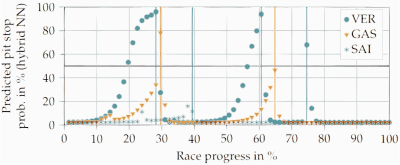
\includegraphics[width=0.7\textwidth]{assets/figures/vse_hnn.png}
        \caption{\label{vse_ffnn}Progression des probabilités d'arrêt au stand pour trois pilotes prédites par le réseau feed-forward, le réseau récurrent et le réseau hybride en utilisant des données du Grand Prix du Brésil 2019, figure repris du papier "Virtual Strategy Engineer: Using Artificial Neural Networks for Making Race Strategy Decisions in Circuit Motorsport"}
    \end{center}
\end{figure}

Les 2 travaux "Tire Changes, Fresh Air, and Yellow Flags: Challenges in Predictive Analytics for Professional Racing" \cite{doi:10.1089/big.2014.0018} et "Real-time decision making in motorsports : analytics for improving professional car race strategy"\cite{phdthesis}
sont des équivalences à notre problématique appliquée au monde de la NASCAR. La NASCAR est une course compétition américaine sur circuits ovales avec des voitures de série modifiées,
dans ce contexte, met davantage l'accent sur les courses en peloton, les dépassements sont plus fréquents et le ravitaillement en carburant est un facteur stratégique majeur.
Ils apportent cependant une formulation différente intéressante, la variable prédite par ses systèmes est le nombre de positions gagnées ou perdues à la suite d'une décision stratégique.

Finalement, on peut noter l'article “Formula-E race strategy development using distributed policy gradient reinforcement learning” de l'université de Cranfield \cite{LIU2021106781} qui utilise une approche de reinforcement learning pour établir une stratégie.
Cet article présente une méthode de développement de stratégies de course dans le contexte du championnat de Formule E, où les voitures ne changent pas de pneus et où la stratégie est davantage liée à l'économie de la batterie.
Cependant, bien que le contexte soit différent de celui proposé dans ce projet et que l'approche reinforcement learning nécessite une simulation précise, la méthode utilisée reste intéressante à noter.

\section{Méthodologie}
La méthodologie adoptée pour cette thèse comprendra les étapes suivantes. Tout d'abord, une analyse approfondie des données disponibles sera réalisée afin d'acquérir une connaissance approfondie de la problématique étudiée.
Ensuite, plusieurs formulations du problème, modèles et méthodes seront explorés à travers des expérimentations.
Les performances respectives de ces approches seront mesurées à l'aide de différentes métriques pour confirmer leur adéquation avec l'objectif fixé.
\chapter{Données}
Cette section est consacrée à l'étude des données disponibles sur les courses de Formule 1 et à la création d'un dataset adapté
à l'entrainement d'un modèle de Machine Learning.

\section{Données existantes}

Il existe 2 principales sources de données disponibles sur les courses de Formule 1.
La première est le dataset Ergast, qui est un projet open source qui répertorie des données sur les résultats des Grand Prix.
La seconde est la Formule 1 elle-même qui diffuse publiquement une certaine partie des données, dites "Live Timing",
qui correspondent aux données des capteurs des voitures.
Les données ont donc plusieurs temporalités :
\begin{itemize}
    \item les informations sur un weekend de courses (circuit, saison, etc.)
    \item les données pour un tour de course (temps au tour, gomme de pneu, etc.)
    \item les données des capteurs (vitesse, distance avec les autres voitures, etc.)
\end{itemize}

FastF1 est une librairie Python qui permet facilement d'accéder aux données de l'API Ergast et aux données officielle de la Formule 1 depuis 2018.
\fig[H, width=0.9\textwidth]{Diagramme en couches des données}{data_layers.svg}

La quantité entre les catégories de données que nous avons surnommés respectivement données de courses, données de tour et données de télémétrie
sont très différentes.

\fig[H, width=0.9\textwidth]{Nombre de données par courses, pour chaque catégorie de données}{nbSamples.svg}

\subsection{Données de courses}
Ces données donnent des informations sur le weekend de course et ne changent pas au cours de ce dernier.
La majorité des features de cette catégorie sont connues pendant la course et donc au moment de l'inférence.

\begin{table}[h]
    \begin{center}
        \caption{Liste d'exemple de features 'données de courses'}
        \begin{tabular}{l|l}
            Nom de la feature & Exemple de valeur \\ \hline
            season            & 2021              \\
            circuit           & Monaco            \\
            number of laps    & 78
        \end{tabular}
    \end{center}
\end{table}

Les autres features sont liées au résultat de la course et ne serais pas disponibles pendant la prédiction.
Mais elles pourraient être utilisées pendant l'entrainement pour par exemple pondérer plus fortement
les stratégies de voitures qui ont de meilleurs résultats.
\subsection{Données de tour}
L'API de la Formule 1 permet d'écouter un flux de données dit "Live Timing".
Ce flux contient différents canaux :
\begin{table}[H]
    \begin{center}
        \caption{Liste des différents canaux fournis dans le flux de données "Live Timing"}
        \begin{tabular}{l|l}
            Canal           & Description                                            \\ \hline
            LapNumber       & Numéro du tour en cours                                \\
            Driver          & Numéro identifiant du pilote                           \\
            LapTime         & Temps du tour précédent                                \\
            Stint           & Nombre de relais effectués                             \\
            TotalLaps       & Nombre total de tours effectués avec ce set de pneus   \\
            Compound        & Type de pneus utilisé                                  \\
            New             & Indique si le pneu a été neuf au moment de son montage \\
            TyresNotChanged & Signale les arrêts aux stands sans changement de pneus \\
            Time            & Temps écoulé depuis le début de la session             \\
            LapFlags        & Drapeaux survenus pendant le tour
        \end{tabular}
    \end{center}
\end{table}

À chaque instant, seulement certains canaux sont actifs. La librairie FastF1 effectue le travail de les agréger sur le parcours d'un tour. Et permet de récupérer ses informations pour tous les tours effectués.
Il serait donc possible de s'abonner à ce flux de donner et d'envoyer directement les informations
émises en entrée du système de prédiction. Un exemple du flux est présenté dans la Table \ref{Live Timing} en annexe.

\subsection{Données de télémétrie}
L'API de la Formule 1 émet également un flux de données pour les données des capteurs des voitures et des capteurs météorologiques.
Les données des capteurs sont envoyés a travers 2 différents flux "Car data" et "Position data" avec des mesures qui sont envoyées environ toutes les 240 millisecondes.
\begin{table}[H]
    \begin{center}
        \caption{Liste des différents canaux fournis dans le flux de données "Car data"}
        \begin{tabular}{l|l}
            Canal    & Description                                                            \\ \hline
            Time     & Temps écoulé depuis le début de la session                             \\
            Date     & Date exacte de la prise de l'échantillon                               \\
            Speed    & Vitesse de la voiture en Km/h                                          \\
            RPM      & Régime moteur                                                          \\
            Gear     & Rapport de vitesse                                                     \\
            Throttle & Pression sur l'accélérateur, exprimé en pourcentage de 0 à 100         \\
            Brake    & Indicateur de freinage, Vrai si les freins sont enclenchés, faux sinon \\
            DRS      & Système de réduction de traînée (Drag Reduction System)                \\
                     & Il comporte plusieurs valeurs possibles codifiées :                    \\
                     & 0-1 = désactivé, 8 = éligible, 10-14 = activé
        \end{tabular}
    \end{center}
\end{table}

\begin{table}[H]
    \begin{center}
        \caption{Liste des différents canaux fournis dans le flux de données "Position data"}
        \begin{tabular}{l|l}
            Canal   & Description                                                \\ \hline
            Time    & Temps écoulé depuis le début de la session                 \\
            Date    & Date exacte de la prise de l'échantillon                   \\
            Status  & 'OnTrack' ou 'OffTrack' (en dehors des limites du circuit) \\
            X, Y, Z & Coordonnées de position relative en mètre
        \end{tabular}
    \end{center}
\end{table}

Pour chaque tour de course d'une voiture, il y a alors entre ~300 et 1'000 échantillons de données télémétriques en fonction de la longueur du circuit.
Ces données offrent un aperçu de la performance de la voiture et permettrait d'estimer la performance du pneumatique.
Un exemple de données télémétriques échantillonnées sur un tour de course est donné en figure \ref{telemetry_example}.
\fig[H, width=0.9\textwidth]{\label{telemetry_example} Exemple de données de télémétrie d'un tour de Carlos Sainz au Grand Prix de Grande-Bretagne 2021}{telemetry_example.svg}

\section{Création d'un dataset}

La première expérience est de créer un classificateur binaire (entrée au stand ou pas) qui prends en entrée les informations d'un seul tour de course.
Dans ce contexte, nous avons décidé de discrétiser chaque course en tour pour chaque voiture.
Une course de 50 tours engendre alors 50 x 20 entrées dans la base de données si les 20 voitures terminent la course.

Le sous-ensemble des champs considérés est présentée en table \ref{dataset_features}. Ces variables retenues résultent d'une phase de sélection dans laquelle
les variables redondantes ou estimées comme non prédictive ont été éliminées.

\begin{table}[H]
    \begin{center}
        \caption{\label{dataset_features}Champs retenus dans le dataset}
        \begin{tabular}{ll}
            Champ                   & Description                                      \\ \hline
            LapNumber               & Numéro du tour en cours                          \\
            LapTime                 & Temps du tour en secondes                        \\
            DriverNumber            & Numéro unique du pilote                          \\
            Team                    & Nom de l'écurie                                  \\
            Compound                & Composé de pneu utilisé (soft, medium ou hard)   \\
            TyreLife                & Âge des pneus en nombre de tours                 \\
            TotalLaps               & Nombre de tours totaux de la course              \\
            Track                   & Nom du circuit                                   \\
            TrackStatus             & Drapeaux de course apparaissant pendant le tour  \\
            Stint                   & Nombre de relais effectués                       \\
            DistanceToDriverAhead   & Distance en mètre avec la voiture devant         \\
            DriverAhead             & Numéro unique du pilote devant                   \\
            NumberOfPitStops        & Nombre d'arrêts au stand déjà éffectuées         \\
            Position                & Position dans la course                          \\
            GapToLeader             & Distance en secondes avec le pilote en tête      \\
            IntervalToPositionAhead & Distance en secondes avec le pilote devant       \\
            LapsToLeader            & Nombre de tours de retard avec le pilote en tête \\
            PitStatus               & In Lap / Out Lap / No Pit                        \\
        \end{tabular}
    \end{center}
\end{table}

Pour les données télémétriques qui sont échantillonnées plus d'une fois par tour,
on prend la dernière mesure au moment où la voiture franchit la ligne d'arrivée.
Les tours avec des informations manquantes ont été exclus.
Les saisons 2019 à 2022 compris ont étés considérés, l'année 2023 étant en cours au moment de la rédaction de ce projet
est réservée comme données de test. La base de données contient 87'845 tours de 80 courses et est disponible ici. % TODO link

\section{Exploration des données}
Dans ce chapitre, nous détaillons les modifications apportées aux données pour les préparer à l'entrainement du modèle.
Ainsi que les informations que nous avons pu tirer de l'étude du set de données.

\subsection{Preprocessing}
La feature TrackStatus communiquée dans l'api officielle contient un ensemble d'entier concaténé dans une chaine de caractères où chaque entier représente un drapeau de course agité au cours du tour.
Les différents status et leur entier correspondant sont détaillé dans la table \ref{track_status_table}.
\begin{table}[H]
    \begin{center}
        \caption{\label{track_status_table}Correspondance des status de piste}
        \begin{tabular}{r|l|l}
            Entier & Correspondance       & Description                                    \\ \hline
            1      & Drapeau vert         & La piste est libre                             \\
            2      & Drapeau jaune        & La piste est partiellement bloquée, la course  \\
                   &                      & continue, mais les dépassements sont interdit  \\
                   &                      & dans un ou plusieurs secteurs                  \\
            4      & Voiture de sécurité  & La course est neutralisée, les voitures ne     \\
                   &                      & peuvent pas dépasser, réduisent leur vitesse   \\
                   &                      & et font la queue derrière la voiture de        \\
                   &                      & sécurité                                       \\
            5      & Drapeau rouge        & La course est interrompue, toutes les voitures \\
                   &                      & rentrent au stand                              \\
            6      & Voiture de sécurité  & La course est neutralisée, les voitures ne     \\
                   & virtuelle            & peuvent pas dépasser et réduisent leur         \\
                   &                      & vitesse                                        \\
            7      & Fin de la voiture de & La voiture de sécurité rentre à la fin de ce   \\
                   & sécurité             & tour
        \end{tabular}
    \end{center}
\end{table}

Pour l'utiliser, elle a été transformée en 6 features binaires où chaque feature représente la présence d'un statut.
Les distributions de la variable avant et après la transformation est observable en figure \ref{track_status_plot}.
\fig[H, width=0.9\textwidth]{\label{track_status_plot}Distribution de la feature TrackStatus avant et après la discrétisation}{track_status_binarized.svg}

6'455 observations avait des valeurs manquantes pour les colonnes DriverAhead et DistanceToDriverAhead. En étudiant la distribution des numéros de tour de ces observations,
présentés en figure \ref{hist_missing_driver_ahead}, on remarque que la plupart des tours sont les premiers de la course,
le reste de la distribution est assez uniforme avec une légère diminution de la fréquence après 55 tours, ce qui est logique, car la majorité des courses durent entre 50 et 60 tours.
Les premiers tours de courses seront supprimés du dataset.

\fig[H, width=0.9\textwidth]{\label{hist_missing_driver_ahead}Distribution de la feature LapNumber pour les tours avec des valeurs manquantes}{lap_number_without_driver_ahead.svg}

En figure \ref{gap_leader_missing}, on voit que beaucoup d'échantillons n'ont pas de valeurs pour la colonne GapToLeader et en observants la figure \ref{gap_leader_laps}, on remarque que ce sont tous des voitures qui ont au moins un tour de retard.
Il est difficile et peut intéressant de déterminer l'écart entre une voiture retardataire et le leader, les valeurs manquantes ont donc été remplacées par -1.

\fig[H, width=0.9\textwidth]{\label{gap_leader_missing}Valeurs manquantes de chaque colonne, les observations d'IntervalToPositionAhead nulles sont celles de voiture avec un tour de retard sur tout le peloton, celles avec des valeurs manquantes de DistanceToDriverAhead et DriverAhead sont ceux du pilote en tête.}{null_values_per_column_after_cleaning.svg}

\fig[H, width=0.9\textwidth]{\label{gap_leader_laps}Histogramme de la caractéristique LapsToLeader lorsque GapToLeader est nul}{gap_to_leader_when_laps_to_leader_is_null.svg}

Les features Track et Compound de notre dataset nécessitent un prétraitement avant d'être utilisées dans notre modèle. Nous avons utilisé l'encodage one-hot de la bibliothèque scikit-learn pour effectuer cette transformation.

L'encodage one-hot est une technique couramment utilisée pour représenter des variables catégorielles sous forme de vecteurs binaires.

Par exemple pour la feature Track, en utilisant l'encodage one-hot, on crée des variables binaires pour chaque piste, où une variable est définie à 1 si la course a eu lieu sur cette piste et 0 sinon.

L'utilisation de l'encodage one-hot nous permet de représenter ces caractéristiques catégorielles en évitant d'introduire un ordre ou une relation numérique entre les catégories.

Pour gérer de manière robuste les nouveaux circuits, le OneHotEncoder à été initialisé avec le paramètre handle unknown='ignore'.
De cette manière, le OneHotEncoder ignore simplement les catégories inconnues et génère un vecteur de zéros correspondant à cette catégorie

\subsection{Analyse}

En faisant analyse de forme, le set de données final possède 84'630 lignes et 22 colonnes dont 11 variables quantitatives et 11 qualitatives, la distribution des types de données est en figure \ref{data_types_distribution}.
1'600 lignes ont été supprimées, car elles possédaient des valeurs manquantes, soit environ 2\% du dataset.
\fig[H, width=0.7\textwidth]{\label{data_types_distribution}Distribution des types des features du dataset}{data_types_distribution.svg}

Afin de créer nos deux classes, nous avons utilisé la colonne "PitStatus". Si la valeur de cette colonne est "In Lap", alors la cible "is pitting" est définie comme étant vraie.
La distribution de nos 2 classes, entre au stand sur ce tour ou pas, est extrêmement déséquilibré.
Seulement 3\% de cas positifs uniquement, une attention particulière doit donc être accordée à la gestion de ce déséquilibre
lors de la phase de modélisation afin d'éviter tout biais potentiel.

\begin{table}[H]
    \begin{center}
        \caption{Proportion des valeurs de la target is pitting}
        \begin{tabular}{r|l}
            Négatif & 0.970318 \\
            Positif & 0.029682
        \end{tabular}
    \end{center}
\end{table}

Dans la section suivante, nous examinons la distribution des features du jeu de données.
Seules les plus intéressantes sont présentées ici, les autres seront fournies en annexe \ref{sec:features}.

La distribution en figure \ref{tyreLife_distribution} est unimodal et asymetrique, cela est dû à la nature de l'évolution de l'age des pneumatiques lors de la course.
Supposons que dans une course de 60 tours on effectue des arrêts tous les 20 tours, on a trois périodes distinctes pour les âges des pneumatiques : 1-20 tours, 21-40 tours et 41-60 tours.
Chaque valeur de 1 à 20 apparaîtra trois fois dans la colonne TyreLife.
En revanche, si une voiture ne fait aucun arrêt et parcourt les 60 tours sans changer les pneumatiques, chaque valeur entre 1 et 60 aura seulement un échantillon.

\fig[H, width=0.9\textwidth]{\label{tyreLife_distribution}
    Distribution de la colonne TyreLife
}{TyreLife_distribution.svg}

La distribution de la variable Compound est en figure \ref{compound_distribution}.
On remarque que les pneumatiques les plus utilisés sont les pneumatiques durs et mediums. Les pneumatiques tendres sont utilisés beaucoup moins souvent, ce qui est logique, car ils sont moins durables.
Les intermédiaires et les wets sont utilisés beaucoup moins souvent, car ils ne sont utilisés que dans des conditions météorologiques particulières.

\fig[H, width=0.9\textwidth]{\label{compound_distribution}
    Distribution de la colonne Compound
}{Compound_distribution.svg}

La figure \ref{track_distribution}, présente la distribution de la variable Track.
Track représente le circuit sur lequel la course a lieu, la distribution est assez déséquilibrée, car certains circuits sont plus courts que d'autres se qu'il fait que les pilotes effectuent moins de tours sur ces circuits.
Et d'autre ne sont pas utilisés tous les ans comme le Mugello qui a été utilisé qu'une fois en 2020.


\fig[H, width=0.9\textwidth]{\label{track_distribution}
    Distribution de la colonne Track
}{Track_distribution.svg}
%\input{examples.tex}
\chapter{Expériences}
Au cours de ce travail nous utilisons un apprentissage supervisé, l'idée est d'avoir une approche d'imitation learning.
C'est à dire que les données historiques sont utilisées pour l'entrainement et les décisions prises par les équipes sont considérées comme ground-truth.
On utilise cette méthode car elle nécessite moins de mise en place qu'une approche par renforcement qui nécessiterais la mise en place d'une simulation
pour estimer le temps gagné dans les différents scénarios hypothètiques.
En revanche l'inconvénient de cette méthode est que les modèles ne peuvent pas surpasser les performances des stratégistes étant donnée qu'ils tentent de les copier.
Il est estimé que cela n'est pas un problème dans la mesure où les stratégies employées sont bonnes en moyenne.

\section{Préparation des données}
Les modèles sont entrainés sur les années 2019 à 2022, en réservant l'année 2023 comme set de test afin d'évaluer la capacité du modèle à généraliser
sur des données qui ne sont pas inclus dans le set d'entrainement.
Étant donné la quantité importante de données, nous avons choisi d'effectuer une division du dataset en un jeu d'entraînement et un jeu de validation avec un ratio de 0,2.

Les étapes de preprocessing ont ensuite été appliquée sur les sets de données individuellement afin d'éviter le data leakage.
Ce phénomène se produit lorsque des informations provenant du set de test ou de validation sont incorporées dans le processus d'entraînement du modèle,
ce qui fausse les résultats de l'évaluation et conduit à une estimation optimiste des performances du modèle.

\section{Modélisation}
L'objectif étant de déterminer la stratégie d'une voiture, le problème comporte 2 parties :
\begin{itemize}
    \item La première est de déterminer si la voiture s'arrête ou non.
    \item La seconde est de déterminer les pneus à utiliser si la voiture s'arrête.
\end{itemize}
On peut donc modéliser le problème comme une classification binaire suivie d'une classification multi-classes,
où la première détermine si la voiture s'arrête ou non et la seconde détermine les pneus à utiliser si la voiture s'arrête.
Une autre modélisation possible est de considérer les 2 parties comme un seul problème de classification multi-classes,
où le modèle détermine directement les pneus à utiliser et la classe "ne s'arrête pas" est considérée comme une classe à part entière.
Une dernière modélisation possible est de considérer les 2 parties comme 2 sorties indépendantes d'un même modèle si l'algorithme utilisé le permet.
Les 3 modélisations sont illustrées par la figure \ref{modelisations}.
%TODO : ajouter un schéma pour chaque modélisation

Les modélisations basées sur des modèles de régression sont aussi possibles mais elles ne sont pas considérées car selon l'étude de l'état de l'art
\cite{app10217805} les modèles de classification sont plus performants.

Dans les prochaines sections nous allons détailler les modélisations explorées et les résultats obtenus.
\section{Classification binaire pour la décision d'arrêt}
\subsection{Random Forest}
%La première modélisation explorée est celle d'une classification binaire
%où le modèle considère les informations d'un seul tour de course en entrée et détermine en sortie si la voiture s'arrête ou non à la fin de celui-ci.
Le premier algorithme de classification utilisé est Random Forest, c'est un algorithme d'ensemble qui combine plusieurs arbres de décision.
Il a été choisit car il est performant sur des sets de données déséquilibrés avec mécanisme de pondération des classes et qu'il est interprétable.
L'interprétabilité est un critère important car il permet de comprendre les décisions prises par le modèle se qui vas dans un premier temps nous aider à l'améliorer
et dans un second temps à donner confiance aux utilisateurs du modèle.

L'implémentation utilisée est celle de scikit-learn \cite{scikitLearnRandomForest} qui est une librairie open-source de machine learning pour python.
Les hyperparamètres du modèle ont été choisis après une recherche par grid search avec une validation croisée sur 4 folds.

Grid search est une méthode d'optimisation des hyperparamètres dans laquelle un modèle est entrainé pour chaque combinaison d'hyperparamètres.
Il est donc important de définir une métrique pour estimer la qualité des modèles entrainés.
\subsubsection{Métriques}
Étant donnés, notre set de données très déséquilibré, nous n'allons pas utiliser l'accuracy ou le score ROC AUC car ils ne sont pas adaptés.
Le choix repose entre le F1-score et la balanced accuracy qui sont les 2 métriques les plus communement utilisées pour les sets de données déséquilibrées.

Pour décider quelle métrique favoriser on s'attarde sur leur définition respective à partir des ensembles des classes prédites.
La figure \ref{confusion_diagram} visualise graphiquement ces ensembles pour le cas d'une classification binaire.
\fig[H, width=0.5\textwidth]{\label{confusion_diagram}Visualisation des résultats d'un système de classification binaire}{confusion_matrice.drawio.svg}

La balanced accuracy est définie comme la moyenne entre la sensitivité (rappel) et la spécificité :
$$
    \frac{\text{spécificité}+\text{sensitivité}}{2}
$$
La figure \ref{sensitivity_specificity} visualise les ensembles considérés par la spécificité et la sensitivité.
\fig[H, width=0.4\textwidth]{\label{sensitivity_specificity}Visualisation de la spécificité et de la sensitivité}{sensitivity_specificity.drawio.svg}
la sensitivité ou rappel indique combien de fois le modèle a correctement prédit la classe positive parmi tous les échantillons positifs réels.
La spécificité est l'équivalent de la sensitivité pour la classe négative, elle mesure la proportion d'échantillons négatifs correctement prédits par le modèle.

Le F1-score est défini comme la moyenne harmonique entre la précision et la sensitivité :
$$
    F=2\cdot\frac{\text{précision} \cdot \text{sensitivité}}{\text{précision} + \text{sensitivité}}
$$
La précision indique combien de fois le modèle a correctement prédit la classe positive parmi toutes les prédictions positives faites,
La figure \ref{precision_recall} montre les ensembles considérés par ses 2 métriques.
\fig[H, width=0.4\textwidth]{\label{precision_recall}Visualisation de la précision et de la sensitivité}{precision_recall.drawio.svg}
On peut observer que le F-score pénalise une précision ou un rappel faible, 2 métriques qui ne considèrent pas les vrai négatifs et qui accordent une grande importance à l'identification de la classe positive.
Pour cette raison, le f1 score est souvant utilisé dans les problèmes de détections d'anomalies, car les sets de données sont fortement biasés en faveur de la classe négative.
Notre cas est assez similaire à ce cas de figure avec 97\% de cas négatifs, le f1 score devrait donc être plus adapté.

En utilisant l'implémentation GridSearchCV de scikit-learn, nous avons effectué une optimisation du f1 score, les hyperparamètres sont en table \ref{grid_params}.

\begin{table}[H]
    \begin{center}
        \caption{\label{grid_params}Paramètres de la recherche GridSearchCV}
        \begin{tabular}{r|l}
            hyperparamètre & valeurs                            \\ \hline
            class weight   & None, balanced, balanced subsample \\
            n estimator    & 100, 500, 1000, 2000               \\
            max depth      & 5, 20, None                        \\
            max features   & sqrt, log2, None                   \\
        \end{tabular}
    \end{center}
\end{table}

La table complète des résultats est en annexe \ref{grid_search_results}.

Le meilleur modèle obtient un f1 score de 0.13 avec les paramètres en table \ref{rf_params}.
Ce score est très faible, nous allons étudier les performances du modèle sur le set de validation pour comprendre ce résultat.

\begin{table}[H]
    \begin{center}
        \caption{\label{rf_params}Paramètres du meilleur modèle}
        \begin{tabular}{r|l}
            hyperparamètre & valeur             \\ \hline
            class weight   & balanced subsample \\
            n estimator    & 2000               \\
            max depth      & 5                  \\
            max features   & sqrt               \\
        \end{tabular}
    \end{center}
\end{table}

Les métriques des résultats sont observables en table \ref{rf_results} et la matrice de confusion en table \ref{rf_matrix}.
En raison de la nature déséquilibrée de notre classification, on ne peut pas se fier à la métrique d'accuracy.

\begin{table}[H]
    \begin{center}
        \caption{\label{rf_matrix}Matrice de confusion de l'entrainement du premier modèle, les colonnes représentent les prédictions et les lignes le ground truth.}
        \begin{tabular}{r|cc}
                    & Négatif & Positif \\ \hline
            Négatif & 10470   & 3422    \\
            Positif & 103     & 281     \\
        \end{tabular}
    \end{center}
\end{table}

\begin{table}[H]
    \begin{center}
        \caption{\label{rf_results}Matrice de confusion de l'entrainement du premier modèle, les colonnes représentent les prédictions et les lignes le ground truth.}
        \begin{tabular}{r|ccc}
            Classe  & Precision & Recall & F1Score \\ \hline
            Négatif & 0.99      & 0.75   & 0.86    \\
            Positif & 0.08      & 0.73   & 0.14    \\
        \end{tabular}
    \end{center}
\end{table}

On remarque dans les résultats que le modèle à de la peine à classifier les cas positifs avec beaucoup de faux-positifs.

\subsubsection{Analyse des résultats}
Premièrement, pour confirmer que le modèle utilise correctement les variables pour la décision nous étudions les raisons derrière ses décisions avec des méthodes d'explications.

Random Forest étant un algorithme interprétable, il nous permet de mesurer en figure \ref{feature_importance_rf_pit} l'importance des features dans sa classification.
L'importance d'une feature est calculée comme la réduction totale de l'entropie normalisée apportée par cette feature.
\fig[H, width=0.9\textwidth]{
    \label{feature_importance_rf_pit}Importance des features du modèle de Random Forest pour la classification des arrêts au stand.
}{feature_importance_rf_pit.svg}

Les features TyreLife, LapNumber et Stint sont les plus importantes. Ce qui est cohérent avec nos connaissances sur la stratégie de course.
Les features les moins utilisées sont celles liées au circuit, nous supposons que c'est parce que la feature est one-hot encoded se qui crée une grande matrice creuse
les features individuelles apporte donc peu d'information au modèle.

Pour comprendre les résultats, nous allons analyser les prédictions du modèle sur le set de validation.
Random Forest est un algorithme interprétable localement de lui même mais le grand nombre d'arbre dans notre modèle rend cela plus difficile.
Nous utilisons LIME (Local Interpretable Model-agnostic Explanations) \cite{lime} un outil d'explication locale,
c'est à dire qu'il permet d'expliquer les prédictions pour une instance donnée.
Pour ce faire LIME fonctionne de la manière suivante:
\begin{enumerate}
    \item On génère un ensemble de données autour de l'instance à expliquer en perturbant légerement les features.
    \item On prédit la classe de l'ensemble de données généré avec le modèle.
    \item On entraine un modèle explicable avec comme features l'ensemble de données généré et comme labels les prédictions du modèle. LIME attribue un poids à chaque instance de l'ensemble de données généré en fonction de la distance avec l'instance à expliquer. Les instances les plus proches sont plus importantes car elles sont plus représentatives de l'instance que l'on cherche à expliquer.
\end{enumerate}

Nous allons étudier les décisions prises pendant la course de Lance Stroll au Grand Prix d'Espagne 2023,
on peut observer la progression  des probabilités d'arrêt au stand en figure \ref{stroll_barcelona_2023}.
\fig[H, width=0.9\textwidth]{
    \label{stroll_barcelona_2023}Progression des probabilités d'arrêt au stand pour le Grand Prix d'Espagne 2023 de Lance Stroll.
    Les probabilités sont calculées à chaque tour en utilisant les données du tour précédent.
    Les lignes verticales rouges indiquent la target du modèle, c'est à dire un tour avant l'arrêt au stand réel.
    Les bares horizontales en haut de la figure indique le composé de pneu utilisé (rouge = tendre, jaune = médium, gris = dur).
}{barcelona_2023_lance_stroll.svg}

Le modèle semble capturer la relation entre les arrêts au stand et les données de course.
Les probabilités d'arrêt au stand augmentent à chaque tour et diminuent drastitquement après un arrêt au stand réel.
Les probabilités augmentent également plus faiblement pendant le relai sur pneus durs se qui est cohérent avec la dégradation plus faible de ces pneus.
Cependant le modèle ne semble pas pouvoir augmenter la probabilité d'arrêt au stand assez rapidement pour éviter les faux positifs, cela explique les résultats de la matrice de confusion.
Ces résultats sont cohérents avec les observations de l'étude \cite{app10217805}.

Nous allons maintenant étudier les explications de LIME pour les tours 2, 8 et 16 de cette course.
Premièrement, on peut observer en figure \ref{lime_2} les résultats de LIME pour le tour 2, où le modèle à décidé de ne pas s'arrêter.
\fig[H, width=0.9\textwidth]{
    \label{lime_2}Résultat de l'algorithme d'explication LIME pour le tour 2 de la course de Lance Stroll à Barcelone en 2023.
}{explanation_barcelona_stroll_2.svg}

On peut voir que l'age des pneus faible est la raison principale de la décision. En figure \ref{lime_8} les résultats de LIME pour le tour 8, le premier tour où le modèle décide de s'arrêter.
\fig[H, width=0.9\textwidth]{
    \label{lime_8}Résultat de l'algorithme d'explication LIME pour le tour 8 de la course de Lance Stroll à Barcelone en 2023.
}{explanation_barcelona_stroll_8.svg}

L'age des pneus a augmenté et sont impact négatif sur la décision est plus faible. L'absence de pneumatique dur et le fait que la voiture soit dans son
premier relai sont les raisons principales de la décision. En figure \ref{lime_16} les résultats de LIME pour le tour 16, le premier tour après l'arrêt au stand.
\fig[H, width=0.9\textwidth]{
    \label{lime_16}Résultat de l'algorithme d'explication LIME pour le tour 16 de la course de Lance Stroll à Barcelone en 2023.
}{explanation_barcelona_stroll_16.svg}
La prédiction est redevenue négative car l'age des pneus est de nouveau faible. De plus, on peut observer l'impact négatif sur la prédiction du second relai.
Le modèle a appris que les voitures font au moins deux relais il est donc normal que le second relai ait un impact négatif sur la prédiction.
Dans l'ensemble, les features utilisées par le modèle sont cohérentes avec nos connaissances sur la stratégie de course.

Pour étudier le comportement du modèle face au périodes de safety car, on observe la progression des probabilités d'arrêt au stand pour le Grand Prix d'Azerbaïdjan 2023 de Sergio Perez en figure \ref{baku_2023}.

\fig[H, width=0.9\textwidth]{
    \label{baku_2023}Progression des probabilités d'arrêt au stand pour le Grand Prix d'Azerbaïdjan 2023 de Sergio Perez.
    Les zones jaunes indiquent les périodes de drapeau jaune, de safety car ou de virtual safety car.
}{baku_2023_sergio_perez.svg}

La période de drapeau jaune au tour 10 a poussé le modèle à prédire un arrêt au stand pour Sergio Perez.
Ce qui est cohérent avec la stratégie de course de l'équipe Red Bull qui a effectué un arrêt au stand pour Sergio Perez au tour 11.
En figure \ref{lime_baku_10} on peut observer les résultats de LIME pour le tour 10, le drapeau jaune est la raison principale de la décision.
\fig[H, width=0.9\textwidth]{
    \label{lime_baku_10}Résultat de l'algorithme d'explication LIME pour le tour 10 de la course de Sergio Perez à Bakou en 2023.
}{explanation_baku_10.svg}

Cependant la période de drapeau jaune au tour 49 a également poussé le modèle à prédire un arrêt au stand alors qu'il n'y en a pas eu.
Cela est dû à un manque d'information sur la raison du drapeau jaune. La première période de drapeau jaune est due à un accident et donc est fortement suseptible d'entrainer une voiture de sécurité.
Alors que la deuxième période de drapeau jaune est due à une sortie de piste sans conséquence et donc n'entraine pas de voiture de sécurité.
Ces information ne sont pas disponibles dans les données car elles sont observables uniquement en regardant les images de la course.
En figure \ref{lime_baku_49} on peut voir que le drapeau jaune est encore une fois la cause de la décision.
\fig[H, width=0.9\textwidth]{
    \label{lime_baku_49}Résultat de l'algorithme d'explication LIME pour le tour 49 de la course de Sergio Perez à Bakou en 2023.
}{explanation_baku_49.svg}

\subsection{Réseaux de neurones}
Les réseaux de neurones sont des modèles plus puissant que Random Forest. Nous allons donc les tester sur le problème de prédiction d'arrêt au stand
pour voir si ils sont capables d'obtenir de meilleurs résultats. Pour ce faire nous avons utilisé la libraire Keras \cite{chollet2015keras} qui permet de construire des réseaux de neurones en Python.
Nous avons testés plusieurs architectures de réseaux de neurones et nous avons obtenu les meilleurs résultats avec l'architecture suivante \ref{neural_network_architecture} :
\begin{table}[H]
    \begin{center}
        \begin{tabular}{|c|c|c|}
            Couche             & Nombre de neurones & Fonction d'activation \\
            \hline
            Couche d'entrée    & 64                 & ReLU                  \\
            1ère couche cachée & 64                 & ReLU                  \\
            Dropout            & 0.2                & -                     \\
            2ème couche cachée & 64                 & ReLU                  \\
            Dropout            & 0.2                & -                     \\
            3ème couche cachée & 64                 & ReLU                  \\
            Dropout            & 0.2                & -                     \\
            Couche de sortie   & 1                  & Sigmoid               \\
        \end{tabular}
    \end{center}
    \caption{Architecture du réseau de neurones utilisé pour la prédiction d'arrêt au stand.}
    \label{neural_network_architecture}
\end{table}

Les couches Dropout sont des couches qui désactivent aléatoirement un certain pourcentage de neurones à chaque itération.
Le réseau de neurones est donc obligé de s'adapter à l'absence de certains neurones et ne peut pas se reposer sur un seul neurone.
Cela nous permet de réduire l'overfitting du modèle et d'améliorer sa capacité de généralisation.
Nous avons également utilisé la technique de Early Stopping qui permet d'arrêter l'entrainement du modèle si la performance sur le jeu de validation ne s'améliore plus.
Nous avons choisi une batch size assez grande de 256 pour s'asssurer que chaque batch contiennent des arrêts au stand.
Comme avec les Random Forest, nous avons réservé 20\% des données pour le jeu de validation et nous avons entrainé le modèle sur les 80\% restants.
Vous pouvez retrouver en table \ref{neural_network_hyperparameters} les hyperparamètres utilisés pour l'entrainement du modèle.
\begin{table}[H]
    \begin{center}
        \begin{tabular}{|c|c|}
            Hyperparamètre & Valeur              \\
            \hline
            Optimizer      & Nadam               \\
            Loss           & Binary Crossentropy \\
            Learning rate  & 0.001               \\
            Epochs         & 300                 \\
            Batch size     & 256                 \\
        \end{tabular}
    \end{center}
    \caption{Hyperparamètres utilisés pour l'entrainement du réseau de neurones.}
    \label{neural_network_hyperparameters}
\end{table}
Pour palier au problème de déséquilibre des classes, nous avons utilisé l'argument class\_weight de la fonction fit de Keras.
Cet argument permet de donner un poids à chaque classe pour le calcul de la loss. Les poids des classes ont étés calculés avec la méthode compute\_class\_weight \cite{classweight}
de la librairie scikit-learn. Les pondérations résultantes sont 0.5 pour la classe 0 et 17 pour la classe 1.

Nous avons obtenu les résultats suivants en table \ref{neural_network_results} avec la matrice de confusion en figure \ref{neural_network_confusion_matrix} :
\begin{table}[H]
    \begin{center}
        \caption{\label{neural_network_confusion_matrix}Matrice de confusion du réseau de neurones.}
        \begin{tabular}{r|cc}
                    & Négatif & Positif \\ \hline
            Négatif & 10053   & 2665    \\
            Positif & 121     & 247     \\
        \end{tabular}
    \end{center}
\end{table}

\begin{table}[H]
    \begin{center}
        \caption{\label{neural_network_results}Métriques de performance du réseau de neurones.}
        \begin{tabular}{r|ccc}
            Classe  & Precision & Recall & F1Score \\ \hline
            Négatif & 0.99      & 0.79   & 0.88    \\
            Positif & 0.08      & 0.67   & 0.15    \\
        \end{tabular}
    \end{center}
\end{table}
Les résultats sont très similaires à ceux obtenus avec les Random Forest. Mais en étudiant le comportement du modèle sur les données de validation,
nous avons remarqué un meilleur comportement. En figure \ref{miami_2023_sainz} vous pouvez voir la différence de comportement entre les deux modèles pour la course de Carlos Sainz sur le Grand Prix de Miami en 2023.
\fig[H, width=0.9\textwidth]{
    \label{miami_2023_sainz}Prédiction d'arrêt au stand pour la course de Carlos Sainz sur le Grand Prix de Miami en 2023.
}{miami_2023_sainz.svg}
Ici le modèle de Random Forest commence à prédire des arrêt au stand dès le 8ème tour, alors que le modèle de réseau de neurones ne commence à prédire des arrêts au stand qu'à partir du 14ème.
Le modèle de réseau de neurones semble pouvoir augmenter sa probabilité d'arrêt au stand plus rapidement que le modèle de Random Forest ce qui est un comportement plus utile pour la stratégie de course.
En étudiant les résultats de LIME sur le 8ème tour de la course en figure \ref{miami_2023_sainz_lime_rf} et \ref{miami_2023_sainz_lime_nn},
on peut voir que le réseau de neurones accordre plus d'importance à l'age des pneus -0.3 contre -0.15 pour le modèle de Random Forest.
\fig[H, width=0.9\textwidth]{
    \label{miami_2023_sainz_lime_rf}Résultats de LIME pour le modèle de Random Forest sur le 8ème tour de la course de Carlos Sainz sur le Grand Prix de Miami en 2023.
}{miami_2023_sainz_lime_rf.svg}
\fig[H, width=0.9\textwidth]{
    \label{miami_2023_sainz_lime_nn}Résultats de LIME pour le modèle de réseau de neurones sur le 8ème tour de la course de Carlos Sainz sur le Grand Prix de Miami en 2023.
}{miami_2023_sainz_lime_nn.svg}
Malgré les métriqes de performance similaires, le modèle de réseau de neurones semble avoir un meilleur comportement.

\subsection{Séries temporelles}
Les précédentes expériences utilisaient uniquement le dernier tour pour prédire la probabilité d'arrêt au stand.
Cependant, il sera plus intéressant d'utiliser les données de plusieurs tours car cela permettra de mieux capturer les tendances.

La formulation du problème devient alors une prédiction de séries temporelles.
On considère alors les données des tours comme une séquence.
Cette formulation est plus naturelle car les données sont une discrétisation par tour de données de capteurs qui sont des séries temporelles.
Elles sont enregistrées de façon séquentielle et sont donc naturellement ordonnées et corrélées.

Il faut cependant grouper les données par course et par voiture pour avoir des séquences de données cohérentes.
On peut observer en figure \ref{time_series_example} la nature séquentielle des données pour un sous ensemble de features.
\fig[H, width=0.9\textwidth]{
    \label{time_series_example}Exemple de séries temporelles pour la course de Lewis Hamilton sur le Grand Prix d'Espagne en 2023.
}{time_series_example.svg}

L'étape de préparation des données est plus complexe que pour les modèles précédents.
Il faut maintenant créer des séquences de données de taille fixe à partir des données de chaque course.
Les données des course de chaque voiture doivent être dans le même set de données (entrainement ou validation).
Le processus de séparation des données est le suivant :
\begin{enumerate}
    \item On regroupe les données avec les colonnes \textit{Year}, \textit{RoundNumber} et \textit{DriverNumber} comme clé.
    \item On mélange ces clés puis on les sépare en 80\% pour l'entrainement, 20\% pour la validation.
    \item On crée les 2 sets de données en utilisant les clés séparées.
\end{enumerate}
La séparation n'est plus exactement fidèle au pourcentage spécifié car on sépare les courses et non les tours.
Mais avec notre grand nombre de données cela ne pose pas de problème.
Ensuite, on crée les séquences de données de taille fixe à partir des données de chaque course.
La cible de chaque séquence est la colonne "is\_pitting" du prochain tour,
par exemple, la cibe d'une séquence comprenant les tours de 10 à 15 est la valeur de "is\_pitting" du tour 16.

Pour cette modélisation nous avons utilisé un réseau de neurones récurrents (RNN) avec des cellules LSTM.
Les réseau de neurones récurrents sont un type de réseau de neurones adapté aux séries temporelles.
Les connexions entre les neurones forment des cycles \ref{rnn_example}, ce qui permet d'utiliser les sorties précédentes comme entrées.
Cela permet aux informations passées d'avoir un impact sur les prédictions futures.
\fig[H, width=0.9\textwidth]{
    \label{rnn_example}Exemple de réseau de neurones récurrents.\cite{rnnExample}
}{rnn_example.svg}
Une des limitations des réseaux de neurones récurrents est le "vanishing gradient problem" où les gradients deviennent trop petits pour être utiles.
Les LSTM (Long Short Term Memory) sont une variante des RNN qui permettent de résoudre ce problème.
L'architecture utilisée est en table \ref{lstm_architecture}.
\begin{table}[H]
    \begin{center}
        \caption{\label{lstm_architecture}Architecture du réseau de neurones récurrents.}
        \begin{tabular}{| l | l | l |}
            Couche  & Nombre de neurones & Fonction d'activation \\ \hline
            LSTM    & 64                 & Tanh                  \\
            Dropout & 0.1                &                       \\
            LSTM    & 64                 & Tanh                  \\
            Dropout & 0.1                &                       \\
            Dense   & 64                 & ReLu                  \\
            Dropout & 0.1                &                       \\
            Dense   & 64                 & ReLu                  \\
            Dense   & 1                  & Sigmoid               \\
        \end{tabular}
    \end{center}
\end{table}

Vous pouvez retrouver en table \ref{rnn_hyperparameters} les hyperparamètres utilisés pour l'entrainement du modèle.
Contrairement au réseaux de neurones classiques nous avons observés de meilleures résultats avec un learning rate plus faible et un batch size plus grand.
\begin{table}[H]
    \begin{center}
        \begin{tabular}{|c|c|}
            Hyperparamètre & Valeur              \\
            \hline
            Optimizer      & Nadam               \\
            Loss           & Binary Crossentropy \\
            Learning rate  & 0.0005              \\
            Epochs         & 100                 \\
            Batch size     & 1024                \\
        \end{tabular}
    \end{center}
    \caption{Hyperparamètres utilisés pour l'entrainement du réseau de neurones.}
    \label{rnn_hyperparameters}
\end{table}

On peut voir en table \ref{rnn_matrix} et \ref{rnn_results} les résultats de ce modèle.
\begin{table}[H]
    \begin{center}
        \caption{\label{rnn_matrix}Matrice de confusion du réseau de neurones récurrents.}
        \begin{tabular}{r|cc}
                    & Négatif & Positif \\ \hline
            Négatif & 8914    & 2607    \\
            Positif & 91      & 242     \\
        \end{tabular}
    \end{center}
\end{table}

\begin{table}[H]
    \begin{center}
        \caption{\label{rnn_results}Métriques de performance du réseau de neurones récurrents.}
        \begin{tabular}{r|ccc}
            Classe  & Precision & Recall & F1Score \\ \hline
            Négatif & 0.99      & 0.77   & 0.87    \\
            Positif & 0.08      & 0.73   & 0.15    \\
        \end{tabular}
    \end{center}
\end{table}

On peut observer une très légère amélioration par rapport au modèle précédent. Cependant, le modèle est toujours très biaisé vers la classe négative.
En figure \ref{comparison_rnn} on peut voir la comparaison des modèles sur les données du Grand Prix d'Espagne 2023 de Max Verstappen.
\fig[H, width=0.9\textwidth]{
    \label{comparison_rnn}Comparaison des modèles sur les données du Grand Prix d'Espagne 2023 de Max Verstappen.
}{comparison_rnn.svg} %TODO fix the figure

On peut observer que le modèle récurrent a un comportement similaire au modèle précédent mais avec des prédictions plus confiantes.
Cependant, il semble sujet a des prédictions assez étrange comme en figure %\ref{rnn_prediction}.
% Add weird prediction figure

\section{Classification multi-classes pour le choix des pneus}
Dans cette section nous allons nous intéresser à la classification multi-classes pour le choix des pneus.
Elle serait utilisée en combinaison avec la classification binaire pour la prédiction des arrêts aux stands.
Le but est que une fois une précition positive pour un arrêt aux stands, on puisse prédire le type de pneus qui sera utilisé.

La préparation des données est similaires à la classification d'arrêt aux stands à la différence que la cible est la colonne "NextCompound".
De plus on ne garde que les tours où un arrêt aux stands a eu lieu. On réduit grandement le nombre d'échantillons (environ de 69'400 à 1'900)
mais le problème devient plus simple car les classes sont plus équilibrées, comme on peut le voir en figure \ref{Compound_distribution}.

Comme avec la classification binaire, nous avons expérimenté avec des modèles Random Forest et des réseaux de neurones.
Le modèle Random Forest a été entrainé avec les hyperparamètres en table \ref{rf_hyperparameters_compound}.
\begin{table}[H]
    \begin{center}
        \caption{\label{rf_hyperparameters_compound}Paramètres du meilleur modèle Random Forest pour le choix des pneus.}
        \begin{tabular}{r|l}
            hyperparamètre & valeur             \\ \hline
            class weight   & balanced subsample \\
            n estimator    & 2000               \\
            max depth      & 5                  \\
            max features   & sqrt               \\
        \end{tabular}
    \end{center}
\end{table}
%TODO faire un grid search pour chercher un meilleur modèle

On peut voir en table \ref{rf_compound_matrix} et \ref{rf_compound_results} les résultats de ce modèle.
\begin{table}[H]
    \begin{center}
        \caption{\label{rf_compound_matrix}Matrice de confusion du meilleur modèle Random Forest pour le choix des pneus.
            Les colonnes représentent les prédictions et les lignes les vraies valeurs.}
        \begin{tabular}{r|ccc}
                   & Soft & Medium & Hard \\ \hline
            Soft   & 83   & 7      & 1    \\
            Medium & 59   & 63     & 7    \\
            Hard   & 68   & 27     & 69   \\
        \end{tabular}
    \end{center}
\end{table}
\begin{table}[H]
    \begin{center}
        \caption{\label{rf_compound_results}Métriques de performance du meilleur modèle Random Forest pour le choix des pneus.}
        \begin{tabular}{r|ccc}
            Classe & Precision & Recall & F1Score \\ \hline
            Soft   & 0.71      & 0.70   & 0.70    \\
            Medium & 0.65      & 0.49   & 0.56    \\
            Hard   & 0.9       & 0.42   & 0.57    \\
        \end{tabular}
    \end{center}
\end{table}
Les résultats sont assez particulier, le modèle prédit souvent la classe Soft, on a beaucoup de faux positifs pour cette classe.
La classe Hard est rarement prédite mais quand elle l'est, elle est souvent correcte.
En figure \ref{rf_compound_prediction} on peut voir la comparaison des prédictions du modèle avec les vraies valeurs.
\fig[H, width=0.9\textwidth]{
    \label{rf_compound_prediction}Prédiction du modèle de Random Forest pour le choix des pneus du grand prix d'Espagne 2023 de Max Verstappen.
}{rf_compound_prediction.svg}
En début de course, le modèle prédit la classe Hard se qui fait sens car c'est le pneu le plus résistant sur lequel on serait le plus susceptible de faire un long relais jusqu'à la fin de la course.
Puis en milieu de course le modèle choisit des pneus Medium avant de choisir des pneus Soft à la fin de la course.
Cela semble être un comportement logique pour un pilote qui cherche à faire le moins d'arrêts aux stands possible.

\section{Autre modélisation}
Nous avons expérimentés les autres modélisation dans lesquelles les deux problèmes sont traités en même temps.
En théorie cela permettrait d'avoir un modèle plus performant car les décisions sont liées.
Deux pistes explorées sont celle d'une classification avec 4 classes ou les 2 colonnes "is\_pitting" et "NextCompound" sont combinées en une seule cible
codifiée de la manière suivante :
\begin{table}[H]
    \begin{center}
        \begin{tabular}{r|c}
            Classe                             & Valeur       \\ \hline
            Pas d'arrêt aux stands             & [1, 0, 0, 0] \\
            Arrêt aux stands avec pneus Soft   & [0, 1, 0, 0] \\
            Arrêt aux stands avec pneus Medium & [0, 0, 1, 0] \\
            Arrêt aux stands avec pneus Hard   & [0, 0, 0, 1] \\
        \end{tabular}
    \end{center}
\end{table}

L'autre piste est celle d'un réseau de neurones avec 2 sorties, une pour chaque problème.
L'une des sorties est une classification binaire pour la prédiction des arrêts aux stands soit un seul neurone avec une fonction d'activation sigmoïde.
L'autre sortie est une classification multi-classes pour le choix des pneus soit 3 neurones avec une fonction d'activation softmax.
Chacune des sorties possède sa propre fonction de perte. Une telle architecture est illustrée en figure \ref{two_output_nn}.
\fig[H, width=0.9\textwidth]{
    \label{two_output_nn}Architecture d'un réseau de neurones avec 2 sorties.
}{two_output_nn.svg}

Ces deux pistes n'ont pas donné de résultats concluants. Les modèles sont bien moins performants que ceux présentés dans les sections précédentes.
Cela peut être dû au fait que la sur-représentation de la classe "Pas d'arrêt aux stands" rend difficile l'apprentissage des classes du choix des pneus.

\section{Métrique de performance}
Suite à l'analyse des résultats des différents modèles explorés dans ce chapitre, on a pu observer que
les métriques qui considérait les prédictions comme des résultats booléens (True positif, False positif, ...) étaient assez peu représentatives de la performance des modèles.

En effet, dans son utilisation finale, le modèle n'as pas besoin d'être restraint à une prise de décision binaire avec des seuils de probabilité.
Il peut simplement donner une probabilité d'arrêt aux stands pour chaque tour de la course. C'est alors aux ingénieurs de l'équipe de décider
si ce seuil est suffisamment élevé pour justifier un arrêt aux stands.

Il fait donc plus sens d'utiliser des métriques qui considèrent les prédictions comme des probabilités et qui sont calculées sur l'ensemble des prédictions d'une course,
le scénario d'utilisation du modèle final. L'objectif est de faire la différence entre un modèle ne prédirait pas du tout un arrêt aux stands et un modèle qui l'aurait prédit
avec quelques tours de retard.

La métrique proposée pondère les prédictions d'une course en fonction de leur impact. Les tours où la voiture rentre aux stands, les modèles sont récompensés
proportionnellement à la probabilité d'arrêt prédite.
\chapter{Conclusion}
%%if
Au moment de ce rendu intermédiaire, un premier modèle a été entrainé, il présente des résultats relativement médiocres
mais cohérent avec l'état de l'art actuel dans le domaine.  Cependant, il s'agit maintenant d'entreprendre différentes pistes pour améliorer les prédictions.
Explorer différents algorithmes tel que les réseaux de neurones, notamment les réseaux de neurones récurrents et la modélisation du problème tel qu'un time series.
Analyser les résultats pour découvrir les features les plus prédictives et potentiellement en créer de nouvelles plus informatives.
%%fi

\vfil
\hspace{8cm}\makeatletter\@author\makeatother\par
\hspace{8cm}\begin{minipage}{5cm}
    %%if
    % Place pour signature numérique
    %\printsignature
    %%fi
\end{minipage}

\clearpage
\printbibliography

\appendix
\appendixpage
\addappheadtotoc
\chapter{Première annexe}
\begin{table}[H]
    \begin{center}
        \caption{\label{Paramètres de la simulation}Paramètres de la simulation utilisées pour les examples en introduction}
        \begin{tabular}{l|l}
            $N$                                & 70   \\
            $t_{optimal}$                      & 95   \\
            $t_{penalite}$                     & 0.06 \\
            $p_{depart}$                       & 110  \\
            $d_{per\textit{f}ormance}(tendre)$ & 0    \\
            $d(tendre)$                        & 0.2  \\
            $\delta{d(tendre)}$                & 0.1  \\
            $d_{per\textit{f}ormance(medium)}$ & 0.75 \\
            $d(medium)$                        & 0.08 \\
            $\delta{d(medium)}$                & 0.08 \\
            $d_{per\textit{f}ormance}(dur)$    & 1.5  \\
            $d(dur)$                           & 0.06 \\
            $\delta{d(dur)}$                   & 0.07 \\
            $t_pitstop$                        & 25   \\
            $t_pitstop_safety_car$             & 15   \\
        \end{tabular}
    \end{center}
\end{table}
\begin{landscape}
    \begin{table}[H]
        \begin{center}
            \caption{Flux "\label{Live Timing}Live Timing" de la voiture 31 pendant le Grand Prix de Monaco 2021}
            \begin{tabular}{llllllllll}
                LapNumber & Driver & LapTime         & Stint & TotalLaps & Compound & New & TyresNotChanged & Time            & LapFlags \\ \hline
                2         & 31     & 00:01:20.154000 & 0     & -         & -        & -   & -               & 00:35:51.209000 & 1        \\
                3         & 31     & 00:01:19.421000 & 0     & -         & -        & -   & -               & 00:37:05.565000 & -        \\
                -         & 31     &                 & 0     & 3         & -        & -   & -               & 00:37:05.940000 & -        \\
                4         & 31     & 00:01:18.494000 & 0     & -         & -        & -   & -               & 00:38:24.008000 & -        \\
                -         & 31     &                 & 0     & 4         & -        & -   & -               & 00:38:25.951000 & -        \\
                5         & 31     &                 & 0     & -         & -        & -   & -               & 00:39:42.570000 & -        \\
                -         & 31     &                 & 0     & 5         & -        & -   & -               & 00:39:45.937000 & -        \\
                -         & 31     &                 & 0     & 6         & -        & -   & -               & 00:41:05.970000 & -        \\
                -         & 31     &                 & 0     & 7         & -        & -   & -               & 00:42:20.948000 & -        \\
                8         & 31     & 00:01:17.967000 & 0     & -         & -        & -   & -               & 00:43:37.668000 & -        \\
                -         & 31     &                 & 0     & 8         & -        & -   & -               & 00:43:40.948000 & -        \\
                9         & 31     &                 & 0     & -         & -        & -   & -               & 00:44:56.051000 & -        \\
                -         & 31     &                 & 0     & 9         & -        & -   & -               & 00:45:00.953000 & -        \\
                -         & 31     &                 & 0     & 10        & -        & -   & -               & 00:46:15.975000 & -        \\
                11        & 31     & 00:01:17.770000 & 0     & -         & -        & -   & -               & 00:47:32.098000 & -        \\
                -         & 31     &                 & 0     & 11        & -        & -   & -               & 00:47:35.967000 & -        \\
                12        & 31     & 00:01:17.677000 & 0     & -         & -        & -   & -               & 00:48:49.775000 & -
            \end{tabular}
        \end{center}
    \end{table}
\end{landscape}

\chapter{Deuxième annexe\label{sec:features}}

\fig[H, width=0.9\textwidth]{
    Distribution de la colonne LapNumber.
    On remarque que la distribution est très uniforme, car la variable augmente linéairement au fil de la course.
    On remarque par contre qu'elle est asymétrique, car certaines voitures ne terminent pas la course et certaines courses sont plus longues que d'autres.
}{LapNumber_distribution.svg}

\fig[H, width=0.9\textwidth]{
    Distribution de la colonne LapTime.
}{LapTime_distribution.svg}

\fig[H, width=0.9\textwidth]{
    Distribution de la colonne Stint.
    Elle est similaire à celle de TyreLife pour les mêmes raisons.
}{Stint_distribution.svg}

\fig[H, width=0.9\textwidth]{
    Distribution de la colonne NumberOfPitStops.
    Elle est identique à Stint car NumberOfPitsStops = Stint - 1.
}{NumberOfPitStops_distribution.svg}

\fig[H, width=0.9\textwidth]{
    Distribution de la colonne Position.
    Elle est uniforme avec une asymétrie à droite en raison des voitures qui se retirent avant la fin des courses.
}{Position_distribution.svg}

\fig[H, width=0.9\textwidth]{
    Distribution de la colonne GapToLeader,
    La distribution est très concentrée autour de 0 étant donné que le leader de la course est toujours à 0.
    La distribution est très asymétrique à droite, ce qui est logique, car la plupart des pilotes sont assez près du leader au début de la course.
}{GapToLeader_distribution.svg}

\fig[H, width=0.9\textwidth]{
    Distribution de la colonne DistanceToDriverAhead.
}{DistanceToDriverAhead_distribution.svg}

\fig[H, width=0.9\textwidth]{
    Distribution de la colonne LapsToLeader
}{LapsToLeader_distribution.svg}

\fig[H, width=0.9\textwidth]{
    Distribution de la colonne TotalLaps
}{TotalLaps_distribution.svg}

\chapter{Troisième annexe}

\begin{table}[H]
    \begin{center}
        \caption{\label{grid_search_results}Résultats du GridSearchCV pour le modèle RandomForestClassifier optimisant le score F1.}
        \begin{tabular}{llllll}
            rang & class weight       & max depth & max features & n estimators & score    \\
            1    & balanced subsample & 5.0       & sqrt         & 2000         & 0.130011 \\
            2    & balanced           & 5.0       & sqrt         & 500          & 0.129973 \\
            3    & balanced subsample & 5.0       & sqrt         & 500          & 0.129856 \\
            4    & balanced subsample & 5.0       & log2         & 2000         & 0.129681 \\
            5    & balanced           & 5.0       & log2         & 2000         & 0.129667 \\
            6    & balanced           & 5.0       & sqrt         & 2000         & 0.129547 \\
            7    & balanced subsample & 5.0       & sqrt         & 1000         & 0.129496 \\
            8    & balanced           & 5.0       & sqrt         & 1000         & 0.129489 \\
            9    & balanced subsample & 5.0       & log2         & 1000         & 0.128940 \\
            10   & balanced subsample & 5.0       & log2         & 100          & 0.128932 \\
            11   & balanced           & 5.0       & log2         & 1000         & 0.128561 \\
            12   & balanced subsample & 5.0       & sqrt         & 100          & 0.128288 \\
            13   & balanced subsample & 5.0       & log2         & 500          & 0.127931 \\
            14   & balanced           & 5.0       & log2         & 500          & 0.127563 \\
            15   & balanced           & 5.0       & sqrt         & 100          & 0.127500 \\
            16   & balanced           & 5.0       & log2         & 100          & 0.126691 \\
            17   & balanced subsample & 5.0       & None         & 2000         & 0.122646 \\
            18   & balanced subsample & 5.0       & None         & 1000         & 0.122618 \\
            19   & balanced           & 5.0       & None         & 2000         & 0.122528 \\
            20   & balanced           & 5.0       & None         & 1000         & 0.122481 \\
            21   & balanced subsample & 5.0       & None         & 100          & 0.122207 \\
            22   & balanced subsample & 5.0       & None         & 500          & 0.122206 \\
            23   & balanced           & 5.0       & None         & 500          & 0.122176 \\
            24   & balanced           & 5.0       & None         & 100          & 0.121999 \\
            25   & balanced           & 20.0      & log2         & 100          & 0.090315 \\
            26   & balanced           & 20.0      & log2         & 500          & 0.087494 \\
            27   & balanced           & 20.0      & None         & 100          & 0.086376 \\
            28   & balanced subsample & 20.0      & None         & 100          & 0.084230 \\
            29   & balanced subsample & 20.0      & None         & 500          & 0.083750 \\
            30   & balanced subsample & 20.0      & log2         & 2000         & 0.083263 \\
            31   & balanced           & 20.0      & None         & 1000         & 0.083231 \\
            32   & balanced subsample & 20.0      & None         & 1000         & 0.083107 \\
            33   & balanced subsample & 20.0      & None         & 2000         & 0.082549 \\
            34   & balanced subsample & 20.0      & log2         & 500          & 0.082350 \\
            35   & balanced           & 20.0      & None         & 2000         & 0.082121 \\
            36   & balanced           & 20.0      & None         & 500          & 0.081996 \\
            37   & balanced           & 20.0      & log2         & 2000         & 0.081599 \\
            38   & balanced subsample & 20.0      & log2         & 100          & 0.080868 \\
            39   & balanced           & 20.0      & log2         & 1000         & 0.080385 \\
            40   & balanced subsample & 20.0      & log2         & 1000         & 0.078841 \\
            41   & balanced           & 20.0      & sqrt         & 100          & 0.069933 \\
            42   & balanced subsample & 20.0      & sqrt         & 100          & 0.066912 \\
            43   & balanced subsample & 20.0      & sqrt         & 1000         & 0.065213 \\
            44   & balanced subsample & 20.0      & sqrt         & 500          & 0.064601 \\
            45   & balanced subsample & 20.0      & sqrt         & 2000         & 0.063450 \\
            46   & balanced           & 20.0      & sqrt         & 2000         & 0.062764 \\
            47   & balanced           & 20.0      & sqrt         & 1000         & 0.062609 \\
            48   & balanced           & 20.0      & sqrt         & 500          & 0.058491 \\
            49   & balanced           & NaN       & None         & 500          & 0.004496 \\
            50   & balanced subsample & NaN       & None         & 1000         & 0.004484 \\
            51   & balanced subsample & NaN       & None         & 2000         & 0.004476 \\
            52   & balanced           & NaN       & None         & 2000         & 0.004339 \\
            53   & balanced subsample & NaN       & None         & 500          & 0.003473 \\
            54   & balanced subsample & NaN       & None         & 100          & 0.003272 \\
            55   & balanced           & NaN       & None         & 1000         & 0.003261 \\
            56   & balanced           & NaN       & sqrt         & 100          & 0.002188 \\
            57   & balanced           & NaN       & None         & 100          & 0.002000 \\
            58   & balanced subsample & NaN       & log2         & 2000         & 0.000000 \\
            58   & balanced           & NaN       & sqrt         & 2000         & 0.000000 \\
            58   & balanced           & NaN       & log2         & 2000         & 0.000000 \\
            58   & balanced           & NaN       & log2         & 1000         & 0.000000 \\
            58   & balanced           & NaN       & log2         & 500          & 0.000000 \\
            58   & balanced           & NaN       & log2         & 100          & 0.000000 \\
            58   & balanced           & NaN       & sqrt         & 1000         & 0.000000 \\
            58   & balanced subsample & NaN       & log2         & 1000         & 0.000000 \\
            58   & balanced           & NaN       & sqrt         & 500          & 0.000000 \\
            58   & balanced subsample & NaN       & sqrt         & 100          & 0.000000 \\
            58   & balanced subsample & NaN       & sqrt         & 1000         & 0.000000 \\
            58   & balanced subsample & NaN       & sqrt         & 2000         & 0.000000 \\
            58   & balanced subsample & NaN       & log2         & 100          & 0.000000 \\
            58   & balanced subsample & NaN       & log2         & 500          & 0.000000 \\
            58   & balanced subsample & NaN       & sqrt         & 500          & 0.000000
        \end{tabular}
    \end{center}
\end{table}

%%fi

\let\cleardoublepage\clearpage
\backmatter

\label{glossaire}
\printnoidxglossary
\label{index}
\printindex

% Le colophon est le dernier élément d'un document qui contient des notes de l'auteur concernant la mise en page et l'édition du document : il est parfaitement optionnel.
%\input{colophon.tex}

\end{document}
